% Modelo de Trabalhos em LaTeX da UFC
%
% Na criação deste modelo foi tomada como base os modelos de monografia da UECE
% criados por Rudy Matela e Sergio Correia, sem a ajuda deles este trabalho teria sido muito mais
% difícil. Este modelo utiliza o abnTeX e um pacote (ufc.sty) para formatação
% de alguns anexos necessários da UFC (folha de rosto, CIP, epígrafe, ...).
%
% Este documento não clama possuir conformidade de 100\% com as normas de
% trabalhos da UFC. Consulte os guias oficiais.
%
% Agradeço ao Lincoln que contribui com o brasão da UFC.
% Agradeço ao Regis e a Mônica pelas contribuições com relação ao "Lorem
% ipsum"
%
% OBS: O modelo de monografias da UECE criado por Rudy Matela encontra-se
% disponível em: http://matela.com.br/pub/modelo_monografia/
%
% Autor: Diego Victor Simões de Sousa
% Data: 10/06/2011


\documentclass[pnumabnt,normaltoc,espacoumemeio,capchap]{abnt}		
\usepackage[brazil]{babel}
\usepackage[utf8]{inputenc}
\usepackage{abnt-alf}
\usepackage{graphicx}
\usepackage{ufc}
\usepackage{multicol}
\usepackage{listings}
\usepackage{eufrak}
\usepackage{subfig}
\usepackage[T1]{fontenc}
\bibliographystyle{abnt-alf}
\setcounter{secnumdepth}{3}
\setcounter{tocdepth}{3}

% Informações gerais do documento
\autor{Lourena Maria Domingos}
\autorr{CHAGAS, F. F. S.}
\titulo{}
\local{Fortaleza, Ceará}
\cidade{Fortaleza}
\data{2013}
\orientador{Prof. Dr. Herminio Borges Neto}
\coorientador{Profa. Me. Dina Mara Pinheiro}
\codigocip{A000z}{CDD:000.0}

% Descrição para folha de rosto
\comentario{
Dissertação submetida à Coordenação do Curso
de Pós-Graduação em Ciência da Computação da
Universidade Federal do Ceará, como requisito
parcial para a obtenção do grau de Mestre em
Ciência da Computação.
}

\comentarioaprovacao{
Dissertação submetida à Coordenação do Curso
de Pós-Graduação em Ciência da Computação, da
Universidade Federal do Ceará, como requisito
parcial para a obtenção do grau de Mestre em
Ciência da Computação. 
}

% Informações institucionais
\centro{Centro de Ciências}
\departamento{Departamento de Computação}
\curso{Pedagogia}
\instituicao{Universidade Federal do Ceará}

\tipotrabalho{Dissertação}
%\areaconcentracao{Banco de ...}
%\nivel{Mestrado}
%\tituloacademico{Mestre}

\dedicatoria{Aos meus Pais.}
% Epígrafe: citação e autor
\epigrafe{``Ninguém, ninguém\\Verá o que eu sonhei\\Só você meu amor\\Ninguém verá o sonho\\Que eu sonhei''}
\autorepigrafe{Geraldo Azevedo}

% Membros da comissão avaliadora
\bancaum{\ABNTorientadordata\\Universidade Federal do Ceará - UFC\\Orientador}
\bancadois{Prof. Me. Dina Mara Pinheiro\\Universidade Federal do Ceará - UFC\\Co-orientador}
\bancatres{Prof. Me. Mulher\\Universidade Federal do Ceará - UFC}
%\bancaquatro{Prof. Dr. Zé Ninguém\\Universidade Federal do Ceará - UFC}

% Palavras chave
\pcs{Burocracia}{\LaTeX}{Documentos}
\kws{Bureucracy}{\LaTeX}{Documents}

\begin{document}

\capa
\folhaderosto
%\makecippage
\termodeaprovacao

% Dedicatória (Opicional)
\makededicatoria

\pretextualchapter{Agradecimentos}
Agradeço a Fulano de Tal, Beltrano da Silva e Cicrano das Tantas
pela ajuda na produção do template \LaTeX\ do modelo de trabalhos
científicos da UFC.
\pagebreak

\makeepigrafe
\begin{resumo}
Isto é um template de documento em \LaTeX. Este documento tenta se
aproximar o máximo possível da norma de produção de trabalhos
científicos da UFC. Este documento não possui 100\% de fidelidade
com as normas da UFC. Assim, use-o por sua conta e risco.

\palavraschave
\end{resumo}
\pagebreak

\begin{abstract}
This is a template document in \LaTeX. This document tries to bring as much
of the production standard of UFC scientific work. This document does not have 
100\% fidelity to the rules of the UFC. So, use it at your own risk.

\keywords
\end{abstract}

\listadefiguras
%\listadetabelas
\tableofcontents
% \listadesiglas % \sigla{sigla}{Descrição}
% \listadesimbolos % \simbolo{símbolo}{Descrição}



\chapter{Chegada do Formador}

Neste capítulo, apresentaremos uma breve descrição da disciplina, mostrando elementos que caracterizam o formador\textbackslash{}tutor quando este inicia seu trabalho no MM, as atividades desenvolvidas pela equipe de bolsistas, assim como alguns conceitos básicos sobre a temática abordada que é fundamental na compressão do objeto deste estudo, sob a ótica de Young, Borges Neto, Almeida e Perrenoud.

\section{Descrição da Disciplina Educação a Distância}

A Disciplina de Educação a Distância, consta na grade curricular do curso de pedagogia presencial desde o ano de 2003, inicialmente como disciplina optativa passando a ser obrigatória a partir da reforma curricular seguinte. Vinculada ao departamento de estudos especializados, semestralmente é ofertada 4 turmas aos alunos do terceiro período do curso e tem sua carga horaria desenvolvida 75$\%$ a distância e 25$\%$ presencial, assegurada pela portaria do MEC 2.253 (18\textbackslash{}10\textbackslash{}2008), que registra que os cursos de ensino superior federais devem contemplar 20$\%$ de sua oferta com disciplinas que acontecem de forma não presencial.

Conforme os Referencias de Qualidade para a Educação Superior a Distância (MEC, 2007), ``não há um modelo único de EaD. Os programas podem apresentar diferentes desenhos e múltiplas combinações de linguagens e recursos educacionais e tecnológicos'' (p.7).  Desta forma, esse modelo consta de uma equipe composta de dois professores titulares e oito formadores (tutores) estudantes do curso de graduação, bolsistas do MM, conforme Young:

\begin{citacao}
Em outras universidades ou instituições que oferecem educação a distância, é comum a utilização do termo ''tutor'', para denominar os sujeitos que atuam na educação virtual, auxiliando o professor titular; no entanto, essa nomenclatura traz a ideia do profissional que vai organizar a pratica educativa em temos de controlo, e, em sua concepção mais tradicional, é aquele que ''cuida'' do aluno. Sua função é verificar se os alunos estão entregando as atividades nos prazos, se estão entrando no ambiente virtual de educação, entre outras atividades dessa natureza. Esses acompanhamentos são necessários, mas a função dos formadores não se restringem a isso.(p.69)
\end{citacao}

Esta equipe é responsável por toda a execução da disciplina que se desenvolve nos ambientes virtuais \textit{Moodle} e \textit{Teleduc}. Os dois constituem- se de softwares livres, sendo o primeiro um software australiano utilizado pelo mundo inteiro desde 1999 e o segundo desenvolvido pela Universidade Estadual de Campinas, UNICAMP desde 1998, além de atividades realizadas na rede social \textit{Facebook}, através da ferramenta grupos, está que foi criada nos Estados Unidos da América em 2004.

A ideia de utilizar mais de um ambiente é possibilitar ao discente que ele conheça mais de uma plataforma virtual e suas possibilidades, já que esta disciplina é a única que permite a experiência virtual.

Os ambientes virtuais \textit{Moodle} e \textit{Teleduc} estão hospedados no site do laboratório, www.multimeios.ufc.br e clicar no ícone ``virtual multimeios'' conforme indica a imagem abaixo:

\begin{figure}[!ht]
    \centering
    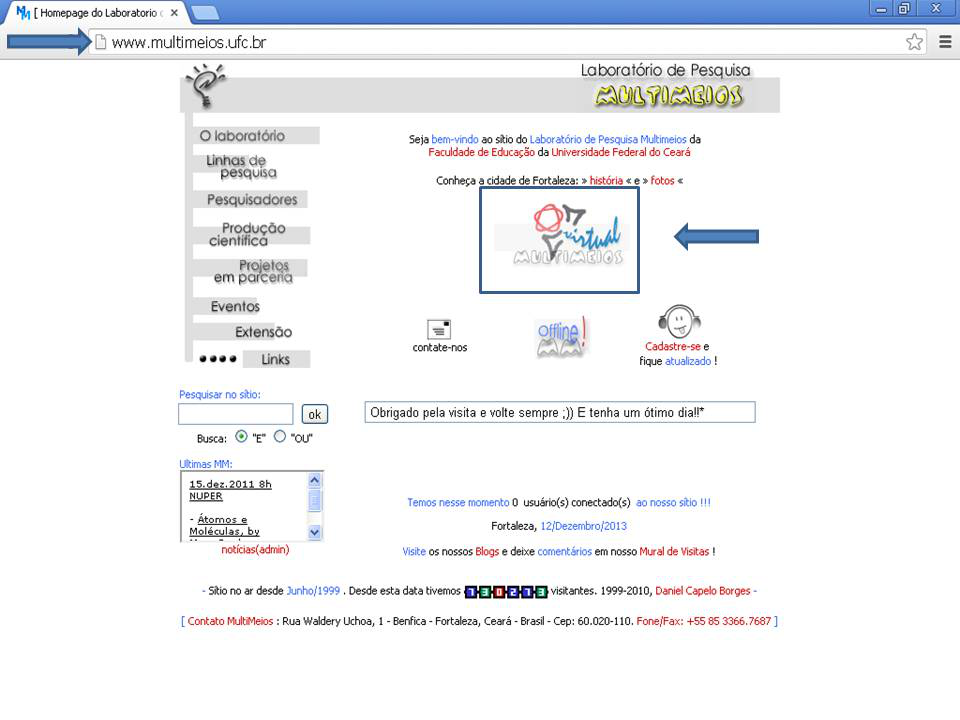
\includegraphics[scale=.5]{f1.png}
    \caption{Caminho para chegar aos ambientes virtuais}
    \label{fig:caminho}
\end{figure}

Esse caminho permite acesso à página de projetos do MM, incluindo os ambientes virtuais citados, que para ter acesso é só clicar no ícone referente a cada um deles:

\begin{figure}[!ht]
    \centering
    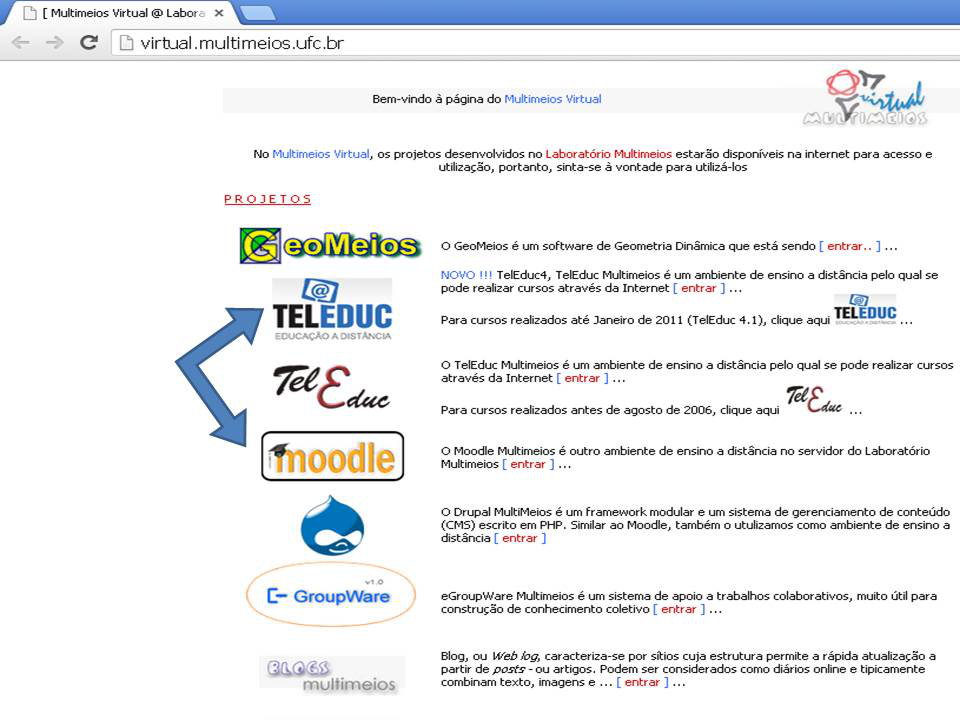
\includegraphics[scale=.5]{f2.png}
    \caption{Página de acesso aos AV’s}
    \label{fig:acessoav}
\end{figure}

Já para entrar no grupo da rede social, os alunos devem fazer login em suas contas pessoais no \textit{Facebook} acessando \underline{www.facebook.com.br} e procurar pelo grupo da disciplina que é sempre divulgado no primeiro dia de aula. Após a solicitação é só aguardar a aprovação de um dos administradores para ter acesso às informações e atividades.

\section{Perfil do Formador}

Pensando em traçar o perfil do formador, apresentaremos quem é esse sujeito e como ele chega a esta condição. 

Para ser formador da disciplina é necessário participar e um processo seletivo que acontece no inicio do ano com a oferta de bolsas para as disciplinas obrigatórias. A seleção consta de duas etapas, sendo a primeira uma prova escrita, seguida de uma entrevista com os professores da disciplina e demais membros do MM. Nesse processo são selecionados dois bolsistas, um remunerado e outro voluntário que serão vinculados ao projeto de monitoria intitulado Formação de mediadores na modalidade à distância. Para participar da seleção é necessário ter cursado a disciplina anteriormente que é, para muitos, o primeiro contato com o ensino a distância, onde é proporcionado a ele a vivência nesta modalidade, então todos os bolsistas ao começar as atividades como formador já trazem o conhecimento prévio sobre a modalidade aprendida enquanto estudante da disciplina.  Os demais formadores são bolsistas do laboratório vinculados a outros projetos que atuam como formadores voluntários com critério também de terem cursado a disciplina anteriormente. Como há uma rotatividade, tendo em vista o processo seletivo, a equipe está sempre se renovando. 

Podemos considerar que neste primeiro momento o bolsista não tem formação para exercer atividades como docentes, e este logo quando chega já vai atuar como formador desenvolvendo atividades junto com os professores, portanto é a partir dessa chegada que começa a formação dos formadores, partindo do principio da ``formação em serviço'', que considera que ao mesmo tempo em que aprende o sujeito também executa, forma enquanto é formado, de forma que assim ele tem um aprendizado contextualizado, que segundo Borges Neto:

\begin{citacao}
Contextualizar conteúdos é reconhecer em primeiro lugar a importância do cotidiano dos/as estudantes no processo educativo e mostrar e demonstrar que os conhecimentos gerados nesse processo de ensino-aprendizagem podem ter aplicação prática na vida das pessoas, de forma geral. Significa compartilhar elementos para que os/as estudantes apreendam o saber, não como armazenamento de conhecimentos técnico-científicos, mas como potencial para enfrentar o mundo de significações e em suas significações.  Borges Neto (2012 p.8)
\end{citacao}

\section{Como funciona a disciplina}

A disciplina é organizada por etapas que começa logo após a seleção dos bolsistas, antes de começar as aulas do semestre, iniciando com a escolha dos materiais e das atividades da disciplina. Nesse momento, toda a equipe se encontra pelo menos duas vezes por semana nas salas anexo ao MM, localizada no prédio NUPER para pensar, organizar e preparar as atividades que serão desenvolvidas ao longo do semestre.

Como não é proposta do laboratório trabalhar com produção de material para a disciplina, durante as primeiras reuniões é solicitado aos formadores, sugestões de textos que possam ser utilizados como referencial teórico no semestre, o material coletado é analisado pela equipe e selecionado. Após a escolha é feito os grupos de estudos onde cada formador apresenta um texto para discutir com o grupo e neste momento propor uma atividade para esse texto e em qual ambiente ela deve acontecer, esta, pode vir a serem umas das atividades do semestre ou se o grupo não concordar, é sugerida outra atividade que se adeque. Desta forma todo o material utilizado no semestre é estudado antes de começar as aulas. Nestas reuniões é produzido o cronograma de atividades, onde se encontra organizado a atividade proposta, o texto base, o prazo para realização e o ambiente aonde irá se desenvolver. Com o cronograma pronto começa a etapa de preparação dos ambientes virtuais. Conforme Almeida 2003, estes:

\begin{citacao}
Permitem integrar múltiplas mídias, linguagens e recursos, apresentar informações de maneira organizada, desenvolver interações entre pessoas e objetos de conhecimento, elaborar e socializar produções tendo em vista atingir determinados objetivos. Almeida (2003, p.331)
\end{citacao}

Para começar a preparação o administrador abre as turmas virtuais, uma em cada ambiente, e cadastra os bolsistas com perfil de formador que confere a eles a possibilidade de manusear como administradores, podendo editar todas as ferramentas, cadastrar os alunos, inserir materiais, preparar e abrir as atividades, entre outros. Com esse perfil o formador tem as mesmas permissões que os professores, permitindo total autonomia com a turma. A equipe se divide e é atribuída funções a cada formador, que pode ser individual ou em duplas, de forma que todas as ferramentas utilizadas sejam contempladas.

É nesse período também que é elaborada a tabela de avaliação com a nota atribuída a cada atividade e os critérios de avaliação. 

\begin{citacao}
A avaliação deve, então, servir de orientação para que o professor possa realizar os ajustes necessários ao seu fazer didático de maneira a transformar as dificuldades em momentos de aprendizagem para seus alunos. Nessa perspectiva, a avaliação torna-se um ``instrumento privilegiado de uma regulação contínua das diversas intervenções e das situações didáticas'' (PERRENOUD, 1999,p.14). 
\end{citacao}

A avaliação perpassa pelas três formas de avaliar em EAD, sendo diagnóstica, formativa e somativa. Diagnóstica, pois no momento em que o aluno chega à disciplina é questionado que conhecimentos ele tem acerca da modalidade, formativa, pois compreende o processo de aprendizagem durante o semestre, considerando os erros do aluno como oportunidade para que ele possa reconstruir seus conceitos, e somativa por que ao final é atribuída nota as atividades que foram produzidas, a fim de obter aprovação curricular.

O contato inicial com os alunos acontece no primeiro dia de aula onde é realizado o primeiro encontro presencial que é apresentado tudo que se refere à disciplina, desde a equipe a atividades que irão ser realizadas e a forma que serão avaliados. Neste momento os alunos realizam seus cadastros nos AV’s e solicitam a inclusão no grupo da rede social. Essas são as primeiras ações que o formador acompanha diretamente os alunos. 

Com os cadastros realizados, os alunos são distribuídos aleatoriamente em grupos, que servem apenas para um acompanhamento mais sistematizado, já que cada grupo é acompanhado por dois formadores. A escolha desta dupla é feita sem tomar como base nenhum critério especifico, só leva em consideração que seja um formador veterano e um formador novato.

Com o inicio do período a equipe continua se encontrando semanalmente para dar continuidade às ações desenvolvidas, que deixa de ser de preparação e passa a ser de execução da disciplina, como ajustes no ambiente virtual, atualização das agendas de acordo com a atividade do momento, se o aluno não conseguir se cadastrar sozinho o formador faz seu cadastro manual, além de discutir e avaliar o andamento da disciplina e o desenvolvimento dos discentes. Há também uma escala de revezamento para atendimento online que acontece através da ferramenta MM Online, que compreende os dias uteis da semana nos turnos tarde e noite. Esta é desenvolvida por Crafty Syntax Live Help (2003 –2009, Eric Gerdes) e adaptada por BORGES NETO, H e BORGES, Daniel Capelo, está alocada no site do Laboratório desde 2006. É semelhante a outras ferramentas de bate-papo, possuindo um layout fácil e com versões disponíveis em diferentes linguagens. 

\section{Percurso de formação do bolsista}

Como dissemos anteriormente essa investigação parte da concepção de formação em serviço, desta forma enquanto atua desenvolvendo as atividades da disciplina, o bolsista formador está sendo formado, desenvolvendo um conjunto de saberes e práticas para atuar com a docência online. Essa formação se fundamenta na proposta teórico metodológica Sequencia Fedathi, que foi desenvolvida pelo grupo FEDATHI na década de 90 e se baseia na aprendizagem por resolução de problemas, levando em consideração a aprendizagem significativa por parte do aluno. É desenvolvida em quatro etapas, tomada de posição, maturação, solução e prova, onde em cada uma delas o professor aparece como mediador na construção do conhecimento por parte do aluno. 

\begin{citacao}
A Sequencia Fedathi, propõe possibilitar ao aluno a elaboração significativa de conceitos, mediante a solução de problemas, cuja as produções serão o objeto sobre o qual o professor vai conduzir a mediação, a fim de levá-lo a construir o conhecimento. Souza (2013 p. 18) 
\end{citacao}

Durante o percurso o formador vivência diversas situações problemas em que os professores participam mediando, sem dar um resposta direta, mas sim levando o formador a pensar na melhor forma de solucionar o problema. Tendo assimilado esse conceito e essa metodologia o formador passa a solucionar sozinho os problemas com os alunos.



%\chapter{Lorem ipsum dolor}
\label{cap:fundamentos}

Lorem ipsum dolor sit amet, consectetur adipiscing elit. Nulla bibendum urna at risus rutrum aliquet. Class aptent taciti sociosqu ad litora torquent per conubia nostra, per inceptos himenaeos. Suspendisse faucibus suscipit lectus id ullamcorper. Cum sociis natoque penatibus et magnis dis parturient montes, nascetur ridiculus mus. Quisque quis nulla eget lorem tincidunt congue. Aenean in augue vitae neque mattis tincidunt. Sed ipsum purus, molestie accumsan porttitor non, blandit ac libero. Proin pharetra purus eget mauris interdum sed congue urna scelerisque. Etiam malesuada, ligula id feugiat feugiat, ligula felis sagittis est, sed tincidunt tortor nisl at dolor. Class aptent taciti sociosqu ad litora torquent per conubia nostra, per inceptos himenaeos. Quisque et sapien ligula. In lacinia lobortis ligula ac consequat. Praesent nisi nisl, lacinia sed lobortis ut, eleifend non quam. Sed eget orci nibh. Aenean vel mi nec libero placerat feugiat. Vivamus leo leo, aliquet ut consectetur eget, vehicula ac urna. Sed convallis, tortor nec porttitor blandit, arcu massa imperdiet lectus, et dictum lorem ligula tempus mi. Nunc non dui massa, nec ultricies purus. Curabitur neque metus, luctus nec tempor ut, egestas ac mauris. Etiam eget mi magna, ac facilisis metus.

Aenean et nunc ut risus pharetra tristique a et purus. Mauris nec rutrum tortor. Aliquam bibendum erat urna, nec volutpat lacus. Proin in nunc lacus. Fusce commodo, orci sit amet adipiscing sollicitudin, libero mauris porttitor mi, quis iaculis nibh elit at sem. Ut aliquet nulla et diam tristique quis egestas odio elementum. Aliquam malesuada faucibus velit, ut pellentesque dui rutrum vel. Quisque faucibus condimentum mi nec varius. Nulla facilisi. Quisque ultricies diam at augue pretium ac ultrices metus pretium. Aenean cursus volutpat augue, ac interdum eros accumsan ut. Class aptent taciti sociosqu ad litora torquent per conubia nostra, per inceptos himenaeos. Sed eu erat nunc, vitae rutrum odio. Maecenas lobortis dignissim enim vel commodo. Nam ut porta ipsum. Nunc convallis auctor massa, quis blandit mauris laoreet eget. Suspendisse a nibh commodo leo dapibus pharetra eget id ante. Donec sit amet justo quis urna laoreet convallis.

Duis volutpat euismod turpis, vitae faucibus risus porta ac. Pellentesque fringilla risus ut mauris fringilla consequat. Nunc porta pulvinar est, ac pulvinar mi gravida ut. Quisque ut nulla erat. Aliquam erat volutpat. Aenean volutpat lacus quis mi ullamcorper eget ultrices augue adipiscing. Pellentesque sed mauris mauris, sit amet porta ipsum. Sed nisl neque, dignissim at rhoncus ac, convallis quis nibh. Nulla adipiscing dapibus odio, eu scelerisque urna ultrices in. Class aptent taciti sociosqu ad litora torquent per conubia nostra, per inceptos himenaeos. Etiam fringilla blandit nulla ut mattis. Phasellus nunc massa, mollis eu venenatis et, porta a tellus. Nam porta, metus at lobortis tempus, augue velit porttitor arcu, cursus mollis nisi mauris at lectus. Suspendisse quis neque mi, faucibus faucibus purus.

\section{Aenean et nunc}
\label{subsec:tbloc}

Aenean et nunc ut risus pharetra tristique a et purus. Mauris nec rutrum tortor. Aliquam bibendum erat urna, nec volutpat lacus. Proin in nunc lacus. Fusce commodo, orci sit amet adipiscing sollicitudin, libero mauris porttitor mi, quis iaculis nibh elit at sem. Ut aliquet nulla et diam tristique quis egestas odio elementum. Aliquam malesuada faucibus velit, ut pellentesque dui rutrum vel. Quisque faucibus condimentum mi nec varius. Nulla facilisi. Quisque ultricies diam at augue pretium ac ultrices metus pretium. Aenean cursus volutpat augue, ac interdum eros accumsan ut. Class aptent taciti sociosqu ad litora torquent per conubia nostra, per inceptos himenaeos. Sed eu erat nunc, vitae rutrum odio. Maecenas lobortis dignissim enim vel commodo. Nam ut porta ipsum. Nunc convallis auctor massa, quis blandit mauris laoreet eget. Suspendisse a nibh commodo leo dapibus pharetra eget id ante. Donec sit amet justo quis urna laoreet convallis.

\subsection{Blih blih blih} 
 
Sed quis euismod massa. Nunc et ultricies nisi. Maecenas feugiat magna eu nibh feugiat gravida. Cras nec leo tincidunt augue porttitor consequat. Vestibulum scelerisque semper augue, tempor ultricies velit pharetra ac. Pellentesque at nunc felis, vitae consectetur dolor. Fusce at turpis augue. Nunc nec lectus odio. Vestibulum non libero purus. In sed enim elit, ut pretium sapien. Curabitur eros risus, pharetra vel vestibulum sed, aliquam ut lacus.


\section{Nullam id tellus}
\label{sec:lateracao}
 
Nullam id tellus velit. Sed vitae sollicitudin mi. Aliquam felis sapien, ullamcorper quis adipiscing at, mollis sed eros. Class aptent taciti sociosqu ad litora torquent per conubia nostra, per inceptos himenaeos. Suspendisse cursus leo at neque egestas in facilisis dui molestie. Proin tincidunt tellus sed enim vulputate aliquam. Morbi placerat nunc eget mi scelerisque in euismod neque accumsan. Aliquam vestibulum volutpat lacus, in dictum quam molestie a. Suspendisse massa lectus, posuere eget tincidunt sed, adipiscing at justo. Nunc scelerisque, elit non posuere semper, lorem magna lacinia justo, et ullamcorper arcu diam non nunc. Pellentesque habitant morbi tristique senectus et netus et malesuada fames ac turpis egestas. Cras vel metus arcu, non venenatis magna. Phasellus viverra lacinia sem ac sagittis. Nullam vel mi nunc, eu congue diam. Praesent rutrum ligula eget tortor posuere ornare. Nullam tempor sem vitae ipsum venenatis eget eleifend libero ultricies. In sagittis euismod aliquam. Cum sociis natoque penatibus et magnis dis parturient montes, nascetur ridiculus mus. Maecenas convallis congue vehicula. Nunc interdum commodo suscipit.



\bibliography{bib}

%\appendix

%\chapter{Isto é um apêndice}

Isto é um apêndice.  Lorem ipsum dolor sit amet, consectetur adipisicing elit,
sed do eiusmod tempor incididunt ut labore et dolore magna aliqua. Ut enim ad
minim veniam, quis nostrud exercitation ullamco laboris nisi ut aliquip ex ea
commodo consequat.  Duis aute irure dolor in reprehenderit in voluptate velit
esse cillum dolore eu fugiat nulla pariatur. Excepteur sint occaecat cupidatat
non proident, sunt in culpa qui officia deserunt mollit anim id est laborum.

\section{Subseção de um apêncice}

Subseção de um apêncice. Lorem ipsum dolor sit amet, consectetur adipisicing
elit, sed do eiusmod tempor incididunt ut labore et dolore magna aliqua. Ut
enim ad minim veniam, quis nostrud exercitation ullamco laboris nisi ut aliquip
ex ea commodo consequat.  Duis aute irure dolor in reprehenderit in voluptate
velit esse cillum dolore eu fugiat nulla pariatur. Excepteur sint occaecat
cupidatat non proident, sunt in culpa qui officia deserunt mollit anim id est
laborum.


\section{Outra subseção de um apêndice}

Outra subseção de um apêndice.  Lorem ipsum dolor sit amet, consectetur
adipisicing elit, sed do eiusmod tempor incididunt ut labore et dolore magna
aliqua. Ut enim ad minim veniam, quis nostrud exercitation ullamco laboris nisi
ut aliquip ex ea commodo consequat.  Duis aute irure dolor in reprehenderit in
voluptate velit esse cillum dolore eu fugiat nulla pariatur. Excepteur sint
occaecat cupidatat non proident, sunt in culpa qui officia deserunt mollit anim
id est laborum.




\end{document}

